\section{Durchf\"uhrung}
\label{sec:Durchfuehrung}
In einem ungeladenen, vertikal ausgerichteten Plattenkondensator wird Öl fein zerstäubt.
Zur Beobachtung der Tröpfchen dient eine Kamera, die mit ausreichender Vergrößerung die Tröpfchen innerhalb des Kondensator sichtbar macht. Der gesamte Versuchsaufbau ist in Abbildung \ref{fig:aufbau} dargestellt.
\begin{figure}
	\centering
	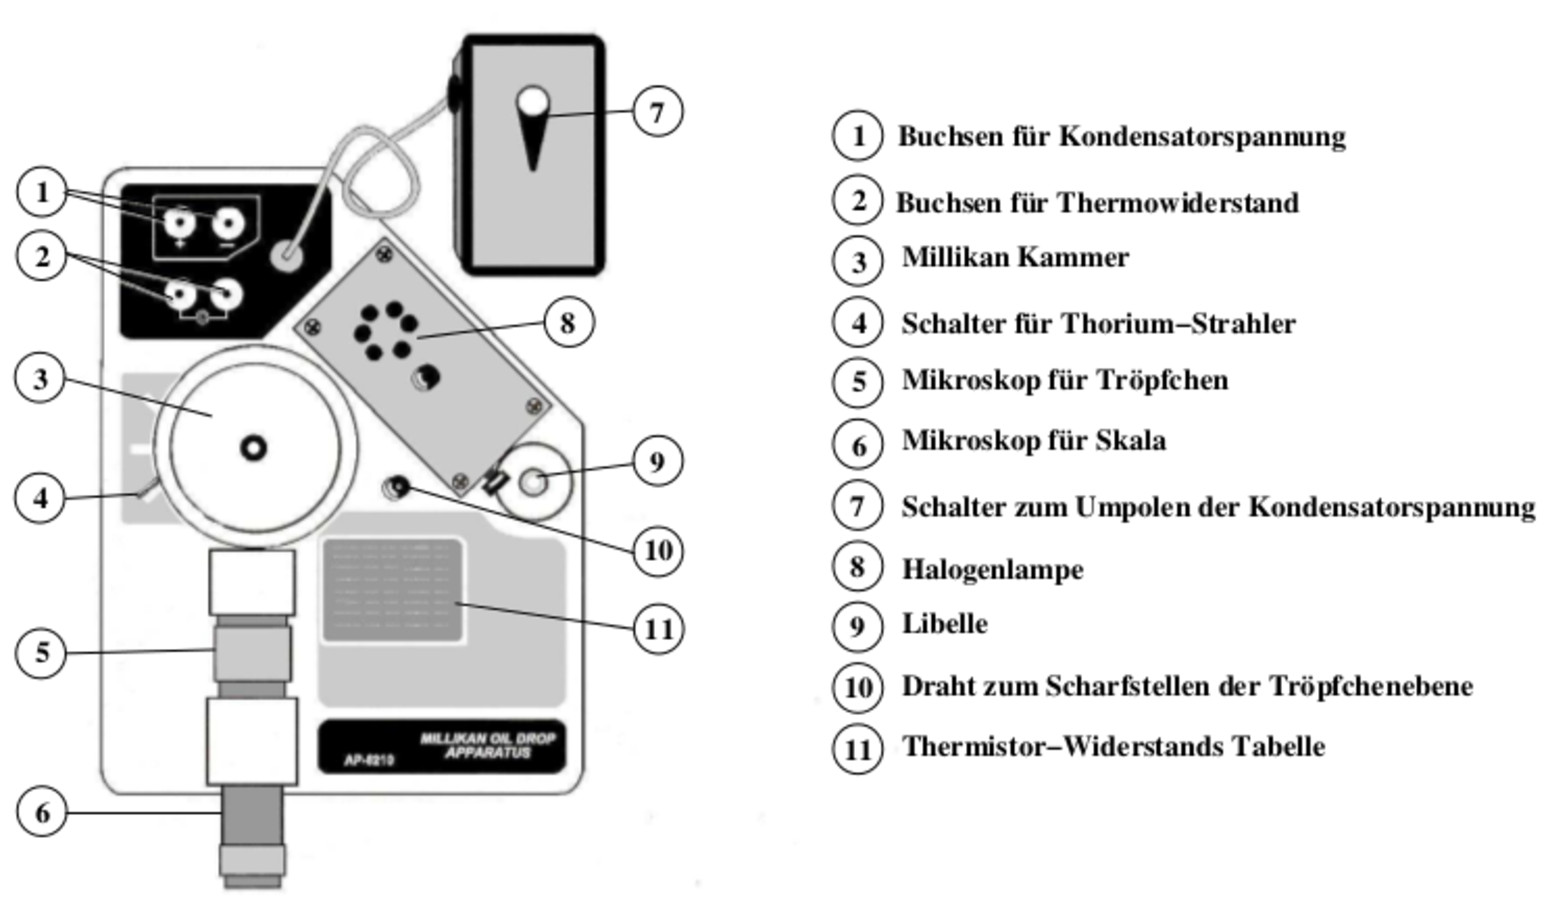
\includegraphics[width=0.7\textwidth]{Bilder/aufbau.pdf}
	\caption{Versuchsaufbau zur Bestimmung der Elementarladung.\cite{skript}}
	\label{fig:aufbau}
\end{figure}
Es wird die Zeit $t$ gemessen, die ein ausgewähltes Tröpfchen zum Überstreichen einer abgemessenen Strecke $s$ benötigt, und  dadurch die Geschwindigkeit $v$ bestimmt.
Ein Teilchen ist als messbar zu betrachten wenn die Horizontalbewegung minimal ist, 
sich die vertikale Grenzgeschwindigkeit $v_0$ ohne Einfluss des elektrischen Feldes in der Größenordnung von $v_0=\SI{0.01}{\centi\meter\per\second}$ bewegt. 
Wichtig ist, dass das Tröpfchen bei der Zerstäubung eine Ladung aufgenommen hat, sodass es auf das elektrische Feld des Plattenkondensators reagiert. Die Horizontalbewegung kann durch Justieren der Apparatur gering gehalten werden.\\
Ist ein messbares Teilchen vorhanden, so wird $t_0$ gemessen um die unbeeinflusste Grenzgeschwindigkeit $v_0$ zu berechnen. 
Anschließend wird bei festgelegter Plattenspannung $U$ die Steig- $t_\text{auf}$ und die Sinkzeit $t_\text{ab}$ unter Einfluss des elektrischen Feldes $E$ gemessen.
Die Messung bei eingeschaltetem Kondensator wird an demselben Tröpfchen mit gleicher Spannung solange wiederholt, bis für jedes Teilchen die Zeiten $t_\text{ab}$ und $t_\text{auf}$ jeweils drei Mal notiert sind.
%Nach der Messung eines Tröpfchens wird mithilfe der Gleichung
%\begin{equation}
%	2\cdot v_0=v_\text{ab}+v_\text{auf}
%	\label{eq:plaus_test}
%\end{equation}
%überprüft, ob das Tröpfchen im Verlauf der Messung die Ladung abgegeben hat und somit für die Auswertung zurückzustellen ist.
Dieses Verfahren wird für vier weitere Tröpfchen unter gleichen Bedingungen wiederholt, sodass für eine angelegte Kondensatorspannung $U$ fünf Messwert-Datensätze von je einem Tröpfchen zur Auswertung bereitstehen.\\
Die Kondesatorspannung $U$ ist zwischen $\SI{200}{\volt}$ und $\SI{300}{\volt}$ zu wählen.
Das Verfahren wird für insgesamt 5 Spannungen durchgeführt.
%Für jedes Teilchen werden insgesamt sieben Zeiten, entsprechend sieben Geschwindigkeiten, gemessen.

Da die Viskosität der Luft von der Temperatur abhängig ist und linear mit ihr ansteigt,
wird während der Messung  die Temperatur in dem Plattenkondensator notiert. Sie wird bestimmt über einen Thermistorwiderstand, welcher über eine Tabelle den zugehörigen Temperaturen zugeordnet werden kann. Eine Temperaturänderung kann vor allem durch die verwendete Halogenlampe hervorgerufen werden, welche die Tröpfchen anstrahlt um sie für die Kamera sichtbar zu machen.

%\subsection{Bestimmung der Elementarladung, des Tröpfchenradius und der Avogadro-Konstanten}
%Der Radius eines Öltröpfchens wird über die Gleichungen \eqref{eq:radius} bestimmt.
%Hierzu wird mit der Temperatur zur Zeit der Messung über Abbildung 
%\ref{fig:temp} die unkorrigierte Viskosität $\eta_\text{Luft}$bestimmt und diese über den Cunningham-Term \eqref{eq:cunningham}
%berichtigt.\\
%Pro Geschwindigkeitspaar $v_\text{auf}$, $v_\text{ab}$  wird nach Gleichung \eqref{eq:ladung} die Ladung $q$ bestimmt und  graphisch aufgetragen, anschließend wird größte gemeinsame Teiler der Ergebnisse bestimmt.

\begin{figure}[h]
	\centering
	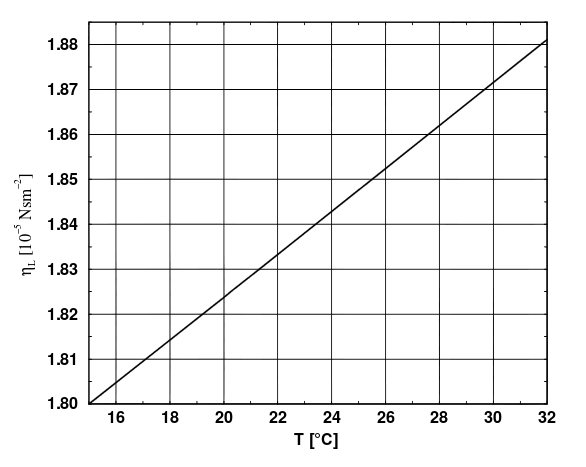
\includegraphics[width=0.8\textwidth]{Bilder/Temp.png}
	\caption{Viskosität der Luft in Abhängigkeit von der Umgebungstemperatur. \cite{skript}}
	\label{fig:temp}
\end{figure}


